\chapter*{ERP Analysis}
\addcontentsline{toc}{chapter}{3. ERP Analysis}
Our first analysis of the data followed a strategy similar to the one used in \cite{schaefer_name_2011}.
Schaefer \etal \cite{schaefer_name_2011} used very short stimuli (3.26s) allowing each stimulus to be repeated many times during during the experiment. 
This allowed them to average across hundreds of short trials. 
They then concatenated the grand average ERPs and applied a \ac{PCA}, which resulted in clearly defined spatial features. 
The differences in the time courses of these spatial features allowed for classification of their stimuli. 
We tried to replicate these results, but we had fewer repetitions of our stimuli. 
Therefore, to preserve as much data as possible we used the full length of the trials as opposed to the first 3.26 seconds. 
We computed grand average \acp{ERP}s by aggregating over the full length of all trials (excluding the cue) of the same stimulus from all subjects. 
We then concatenated the grand average \acp{ERP} and applied a \ac{PCA}. 
This resulted in principle components with poorly defined spatial components \autoref{fig:components} (A and B).

In order to preserve even more of the data and we took an alternative approach. 
All of the raw trials were concatenated to create a single, long trial that contained all of the raw EEG information.
We ran a \ac{PCA} on the concatenated raw trials without first calculating an average across trials. 
This produced clearly defined spatial components \autoref{fig:components} (C and D). 
Except for their (arbitrary) polarity the components are very similar across the two conditions, which replicates the results found in \cite{schaefer_name_2011}.

\begin{figure}[t] 
  \begin{center}
    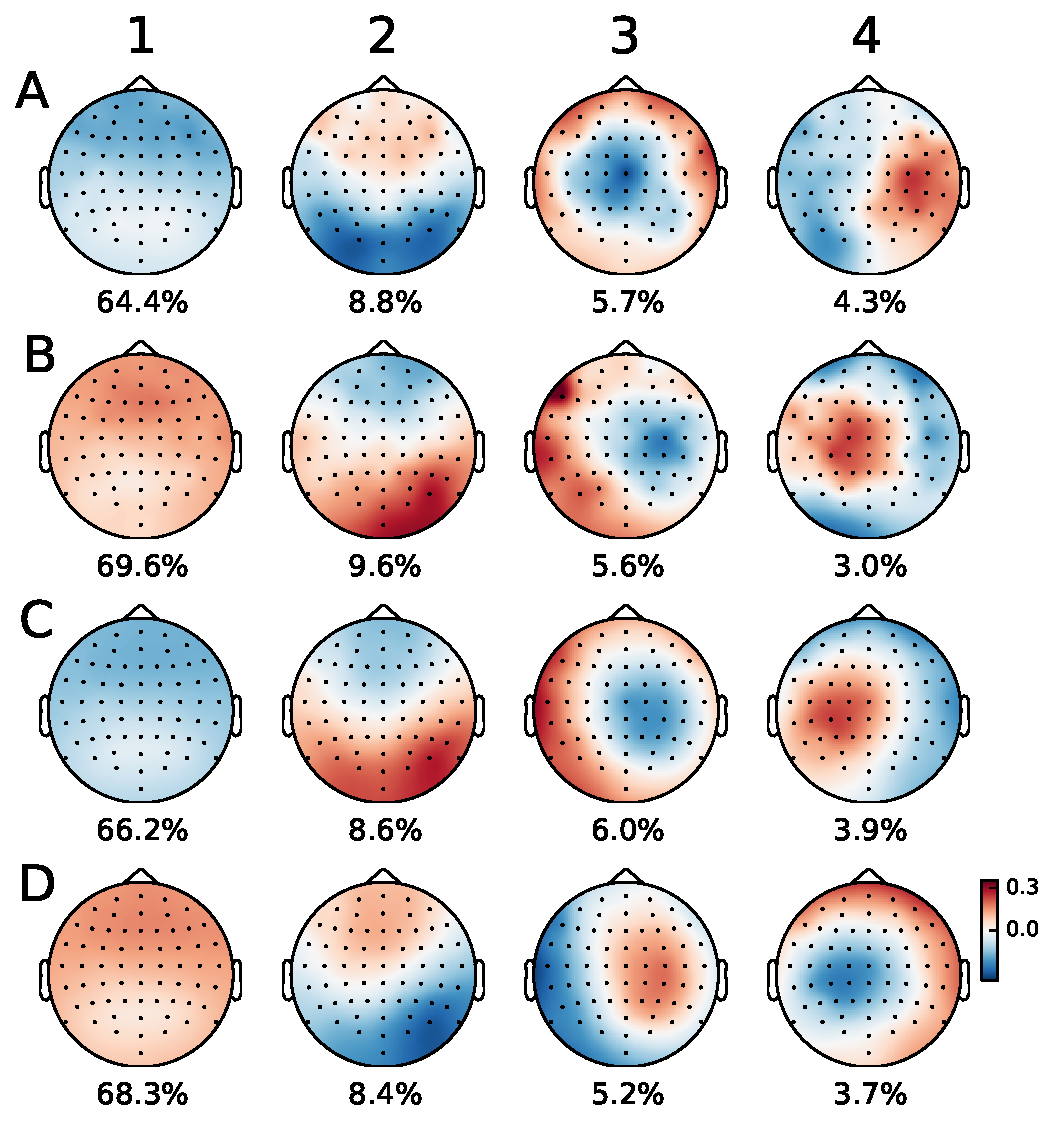
\includegraphics[scale=0.5]{Figures/principle_components.pdf}
    \caption{%
Topographic visualization of the top 4 principle components with percentage of the explained signal variance.
Channel positions in the 64-channel EEG layout are shown as dots.
Colors are interpolated based on the channel weights.
The PCA was computed on
\textbf{A}: the grand average \acp{ERP} of all perception trials,
\textbf{B}: the grand average \acp{ERP} of all cued imagination trials,
\textbf{C}: the concatenated perception trials,
\textbf{D}: the concatenated cued imagination trials.
}
    \label{fig:components}
  \end{center}
\end{figure}

\subsection*{Component Waveform Correlations}
In order to investigate how similar the activation of these components is across conditions and stimuli we took the time course of component three over the first three seconds of each stimulus during perception and imagination and performed a correlation.
We used component three as it accounts for the most variance while being similar to a typical auditory component.
The highest correlations produced by this component is r=0.40 (p$<$0.001) for ``Eine Klein Nachtmusic'' (\autoref{fig:nachtmusic}) and r=0.30 (p$<$0.001) for ``The Emperor Waltz'' (\autoref{fig:emperor}).
Although these correlate well the perception of Eine Kleine Nachtmusic correlates well with the imagination of Jingle Bells without lyrics (r=0.30). 
The highest correlation of r=0.52 (p$<$0.001) occurs between the imagination of Jingle Bells (without lyrics) and the perception of the Star Wars theme \autoref{fig:starjingle}. 
Because high correlations occur between trials from different stimuli we can not use this approach to classify our stimuli.
\hl{include a Table of correlations? with Component 2? component 3?}


\begin{figure}[t]
  \begin{center}
    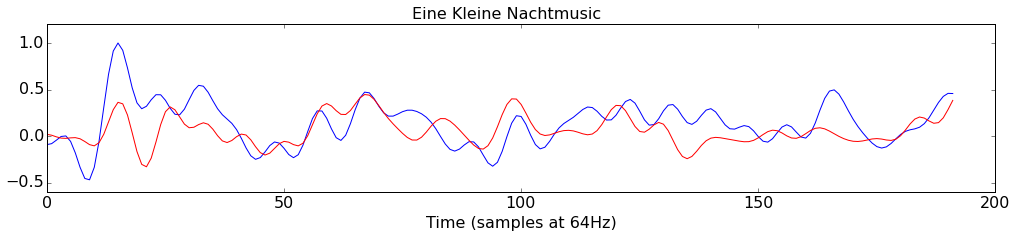
\includegraphics[scale=0.4]{Figures/EineKleineCorrelation}
    \caption{
The time course of component three during perception (blue) and imagination (red) of Eine Kleine Nachtmusic. The correlation between the two time courses is r=0.40 (p$<$0.001).
}
    \label{fig:nachtmusic}
  \end{center}
\end{figure}

\begin{figure}[t]
  \begin{center}
    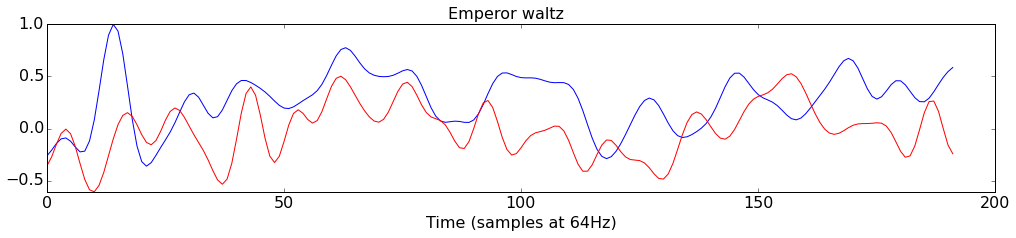
\includegraphics[scale=0.4]{Figures/EmperorCorrelation}
    \caption{
The time course of component three during perception (blue) and imagination (red) of The Emperor Waltz. The correlation between the two time courses is r=0.30 (p$<$0.001).
}
    \label{fig:emperor}
  \end{center}
\end{figure}

\begin{figure}[t]
  \begin{center}
    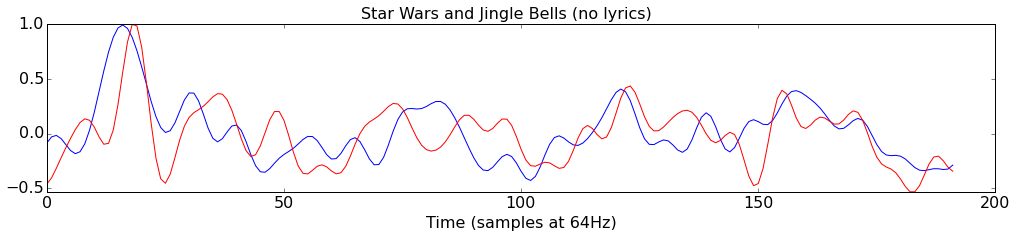
\includegraphics[scale=0.4]{Figures/StarJingle}
    \caption{
The time course of component three during perception (blue) of the Star Wars theme and imagination (red) of Jingle Bells (no lyrics). The correlation between the two time courses is r=0.52 (p$<$0.001).
}
    \label{fig:starjingle}
  \end{center}
\end{figure}

Our inability to accurately classify stimuli using this technique could be caused by our much smaller number of trials which are substantially longer than those used by \cite{schaefer_name_2011}. 
We only had 5 trials per stimulus, ranging from 6.9s to 16s, while Schaefer et al. (2011) collected 145 trials of each of their stimuli each approximately 3s long.